\documentclass[serif]{beamer}

\usetheme[bgphoto]{polimi}

\usepackage{palatino}
\usepackage{eulervm}

% Full instructions available at:
% https://github.com/elauksap/beamerthemepolimi

\usepackage[linesnumbered,lined]{algorithm2e}

\usepackage{amsmath}
\usepackage{mathtools}
\usepackage{bm}
\usepackage{amsthm}
\usepackage{amssymb}
\usepackage{booktabs}

\PassOptionsToPackage{T1}{fontenc} % T2A for cyrillics
    \usepackage{fontenc}

% Set custom font (requires to compile with XeLaTeX).
\usepackage{ifxetex}
\ifxetex
\usepackage{fontspec}
\setsansfont[Scale=0.9]{Arial}
\fi

\newcommand{\atantwo}[2]{\operatorname{atan2}\left(#1, #2\right)}

\usepackage{lipsum}

\title{A ROS implementation of a 6-DoF EKF \\ for indoor drone Visual SLAM}
%\subtitle{Subtitle}
\author{Diego Emanuel Avila}
\date{15-12-2020}

\begin{document}
    \begin{frame}
        \maketitle
        % If the theme option "nologo" is specified, a custom logo
        % can be added with the following commands:
        %\begin{tikzpicture}[overlay, remember picture]
        %    \node at (current page.north) [anchor=north, inner sep=2cm]
        %    {
        %        \includegraphics[width=0.3\paperwidth]{logo_centrato_BN_negativo.png}
        %    };
        %\end{tikzpicture}
    \end{frame}

    \begin{frame}{Table of contents}
        \begin{columns}[t]
            \begin{column}{.5\textwidth}
                \tableofcontents[sections={1-2}]
            \end{column}
            \begin{column}{.5\textwidth}
                \tableofcontents[sections={3-4}]
            \end{column}
        \end{columns}
    \end{frame}

    %%%%%%%%%%%%%%%%%%%%
    % BACKGROUND
    %%%%%%%%%%%%%%%%%%%
    \section{Background}

    \subsection*{Leonardo Drone Contest}
    \begin{frame}
       \begin{itemize}
           \item{Indoor environment}
           \item{Fully autonomous drone}
           \item{No GNSS nor Laser devices}
           \item{Inertial devices, range sensors, cameras and speed sensors are allowed}
           \item{Obstacles
have at most 3mts height with passages of at least 1mt}
           \item{Landmarks: colored poles and QR markers}
           \item{2-phase competition: inspection and path-follow}
       \end{itemize}
    \end{frame}
    \begin{frame}
        \centering
        \includegraphics[width=0.6\linewidth]{Images/fig25-contest-env.png}
    \end{frame}

    \subsection{SLAM}
    \begin{frame}{Simultaneous Localization \& Mapping}
        \begin{columns}[c]
            \begin{column}{.5\textwidth}
                \begin{itemize}
                    \item{Localization: where the robot is}
                    \item{Mapping: build a map of the environment}
                    \item{SLAM: localize itself while building a map}
                \end{itemize}
            \end{column}
            \begin{column}{.5\textwidth}
                \includegraphics[width=\linewidth]{Images/fig27-where-am-i.png}
            \end{column}
        \end{columns}
    \end{frame}
    \begin{frame}
        \centering
        \includegraphics[width=\linewidth]{Images/fig26-slam-a-b.png}
    \end{frame}
    \begin{frame}
        \centering
        \includegraphics[width=\linewidth]{Images/fig26-slam-c-d.png}
    \end{frame}
    \begin{frame}
        \centering
        \includegraphics[width=0.5\linewidth]{Images/fig26-slam-e.png}
    \end{frame}

    \subsubsection{EKF-SLAM}
    \begin{frame}[nonumber]{EKF-SLAM}
         \begin{itemize}
             \item{Motion and observation processes are usually not linear}
             \item{Motion model: $g\left(u_t, \mu_{t-1}\right)$}
             \item{Observation model: $h\left(\hat\mu_t\right)$}
             \item{EKF uses Taylor expansion to linearize the processes}
             \item{Builds feature-based maps}
             \item{The full-state (map) is\\ $\mu = \begin{bmatrix} q_r & m_0 & \dots & m_{n-1}\end{bmatrix}^T$}
             \item{As in Kalman Filter, the process comprises 2 steps: \\prediction and correction}
         \end{itemize}
    \end{frame}

    \begin{frame}
        \begin{columns}[T]
            \begin{column}{.55\textwidth}
                \scalebox{.7}{
                    \begin{algorithm}[H]
                        \DontPrintSemicolon
                        \KwIn{$\mu_{t-1}$, $\Sigma_{t-1}$, $u_t$, $z_t$}
                        \BlankLine
                        $\hat\mu_t = g\left(\mu_{t-1}, u_t\right)$\;
                        $G_t = computeJacobian\left(g\right)$\;
                        $\hat\Sigma_t = G_t \Sigma_{t-1} G_t^T + R_t$\;
                        \BlankLine
                        \ForEach{landmark observation $z_t^i$}{
                            \BlankLine
                            \If{landmark $i$ has not being seen before}{
                                $addLandmarkToStateVector\left( z_t^i \right)$
                            }
                            \BlankLine
                            $H_t^i = computeJacobian\left( h^i \right)$\;
                            $v^i =  z_t^i - h^i \left( \hat\mu_t \right)$\;
                            $S = H_t^i \hat\Sigma_t H_t^{iT} + Q_t$\;
                            $K_t^i = \hat\Sigma_t H_t^{iT} S^{-1}$ \;
                            $\mu_t = \hat\mu_t + K_t^i \left( v^i \right) $ \;
                            $\Sigma_t = (I - K_t^i H_t^i) \hat\Sigma_t$ \;
                        }
                        \BlankLine
                        \Return{$\mu_t$, $\Sigma_t$}
                    \end{algorithm}
                }
            \end{column}
            \begin{column}{.45\textwidth}
               \begin{itemize}
                   \item{Lines 1-4 are the prediction step}
                   \item{Lines 4-14 are the correction step}
                   \item{If the landmark has not being seen before, the algorithm adds it in lines 5-7}
               \end{itemize}
            \end{column}
        \end{columns}
    \end{frame}

    \subsubsection{Adding new landmarks}
    \begin{frame}[nonumber]{New landmarks}
        \begin{itemize}
            \item{Map is not always available}
            \item{Inverse sensor model: $h^{-1}\left(q_r, z\right)$}
            \item{The state vector is extended with $h^{-1}$}
            \item{The covariance matrix is extended as well: \\
                \begin{align*}
                Y_x = \frac{\partial y}{\partial x} = \begin{bmatrix}
                    \frac{\partial x}{\partial x} \\ \frac{\partial h^{-1}}{\partial x}
                \end{bmatrix} = \begin{bmatrix}
                    I \\ G_x
                \end{bmatrix}\\
                Y_z = \frac{\partial y}{\partial z} = \begin{bmatrix}
                    \frac{\partial x}{\partial z} \\ \frac{\partial h^{-1}}{\partial z}
                \end{bmatrix} = \begin{bmatrix}
                    0 \\ G_z
                \end{bmatrix}\\
                \hat{\Sigma} = \begin{bmatrix}
                    \Sigma & \Sigma G_x^T \\
                    G_x \Sigma & G_x \Sigma G_x^T + G_z Q_t G_z^T
                \end{bmatrix}
                \end{align*}
            }
        \end{itemize}
    \end{frame}

    \subsection{NEES}
    \begin{frame}{Normalized Estimation Error Squared}
        \begin{itemize}
            \item{Defined as:
            \begin{align*}
                    NEES = \left(\bm{x} - \hat{\bm{x}}\right) \Sigma^{-1} \left(\bm{x} - \hat{\bm{x}}\right) \le \chi_{d, 1-\alpha}^2
            \end{align*}}
            \item{Can be performed to check the consistency of the filter}
            \item{Consistency of the filter is maintained by using observations that
satisfy the test
                \begin{align*}
                    v^i =  z_t^i - h^i \left( \hat\mu_t \right)\\
                    S = H_t^i \hat\Sigma_t H_t^{iT} + Q_t \\
                    D_i^2 = v^i S^{-1} v^i \le \chi_{d, 1-\alpha}^2
                    \label{eq:chapter2:nees:innov_test}
                \end{align*}
            }
        \end{itemize}
    \end{frame}

    %%%%%%%%%%%%%%%%%%%%
    % IMPLEMENTATION
    %%%%%%%%%%%%%%%%%%%
    \section{Implementation}
    \begin{frame}
        \begin{itemize}
            \item{MAVROS node interfaces with the flight controller, and provides the control signal}
            \item{Control signal is composed by linear and angular velocities
                \begin{align*}
                    u &= \begin{bmatrix} v_x^b & v_y^b & v_z^b & \omega_x^b & \omega_y^b & \omega_z^b & \phi^b & \theta^b & \psi^b \end{bmatrix}^T\\
                    v^w &= \textbf{T} * \begin{bmatrix} v_x^b \\ v_y^b \\ v_z^b \end{bmatrix}
                \end{align*}
            }
        \end{itemize}
    \end{frame}
    \subsection{The drone}
    \begin{frame}{Characteristics}
        \begin{columns}[c]
            \begin{column}{.5\textwidth}
                \begin{itemize}
                    \item{PixHawk 4 Flight Controller}
                    \item{8 range finder}
                    \item{4 monocular cameras}
                    \item{2 stereo cameras: 1 pointing down, 1 pointing forward}
                    \item{1 optical-flow device}
                    \item{Accelerometer + gyroscope}
                    \item{Magnetometer}
                    \item{Barometer}
                \end{itemize}
            \end{column}
            \begin{column}{.5\textwidth}
                \includegraphics[width=\linewidth]{Images/fig28-drone-sim-2.png}
            \end{column}
        \end{columns}
    \end{frame}

    \subsection{Motion model}
    \begin{frame}
        \begin{itemize}
            \item{Given the linear velocities transformation $v^w$, the motion model can be summarized as follow
                \begin{align*}
                    g\left( \mu_{t-1}, u_t \right) = \begin{cases}
                        \begin{bmatrix}
                            \mu_{t-1, x^w} \\ \mu_{t-1, y^w} \\ \mu_{t-1, z^w}
                        \end{bmatrix}
                        + \Delta t * v^w \\
                        \mu_{t-1, \psi} + \Delta t * \omega_z^b
                    \end{cases}
                \end{align*}
            }
        \item{However, this does not consider the noise}
        \end{itemize}
    \end{frame}
    \begin{frame}
        \begin{itemize}
            \item{Noise in the motion process is assumed to be $\mathcal{N}\left(0, R_t\right)$}
            \item{The noise covariance can be decomposed as $R_t = N * U * N^T$
                \begin{itemize}
                    \item{$N$ is the Jacobian of the acceleration with respect to the state vector}
                    \item{$U$ is the average acceleration of the drone}
                \end{itemize}
            }

        \end{itemize}
    \end{frame}

    \subsection{Observation models}
    \begin{frame}
        \begin{itemize}
            \item{2 types of landmarks: Poles \& Markers
                \begin{itemize}
                    \item{Poles' observations is Range and Bearing}
                    \item{Markers' observations is the pose with respect to the camera reference frame}
                \end{itemize}
            }
            \item{Additionally, height correction is done using range sensor and 3D obstacle map}
            \item{Observation for landmark $i$ is $z_i = h_i\left(x_t\right) + \mathcal{N}\left(0, Q_t\right)$}

        \end{itemize}
    \end{frame}

    \subsubsection{Poles}
    \begin{frame}[nonumber]{Poles}
        \begin{itemize}
            \item{Range and bearing information \begin{itemize}
                    \item{$\rho$: distance}
                    \item{$\beta$: altitude}
                    \item{$\alpha$: azimuth}
            \end{itemize}}
            \item{Observation model:
            \begin{align*}
                \begin{bmatrix}
                    p_{i, x}^b \\ p_{i, y}^b \\ p_{i, z}^b
                \end{bmatrix} &= \bm{T_r}^{-1} \begin{bmatrix}
                    p_{i, x}^w \\ p_{i, y}^w \\ p_{i, z}^w
                \end{bmatrix}\\
                h_i(\hat\mu_t) = \begin{bmatrix}
                    p_{i, \rho} \\ p_{i, \alpha} \\ p_{i, \beta}
                \end{bmatrix} &= \begin{bmatrix}
                    \sqrt{ p_{i, x^b}^2 + p_{i, y^b}^2 } \\
                    \atantwo{p_{i, y}^b}{p_{i, x}^b} \\
                    \atantwo{p_{i, z}^b}{p_{i,\rho}^b}
                \end{bmatrix}
            \end{align*}}
        \end{itemize}
    \end{frame}

    \begin{frame}
        \centering
        \includegraphics[width=0.6\linewidth]{Images/fig28-range-and-bearing.png}
    \end{frame}

    \subsubsection{Markers}
    \begin{frame}[nonumber]{Markers}
        \begin{itemize}
            \item{Markers are unknown first, and added to the map once the drone sees them}
            \item{Observations is composed by its position with respect to the camera reference frame}
            \item{Observation model is then: \begin{align*}
                    h_i(\hat\mu_t) = \begin{bmatrix}
                        m_{i, x}^c \\ m_{i, y}^c \\ m_{i, z}^c \\ m_{i, \phi}^c \\ m_{i, \theta}^c \\ m_{i, \psi}^c
                    \end{bmatrix} = (\bm{T_r} * \bm{T_c})^{-1} * \bm{T_m}
                \end{align*}
            }
        \end{itemize}
    \end{frame}

    \begin{frame}
        \centering
        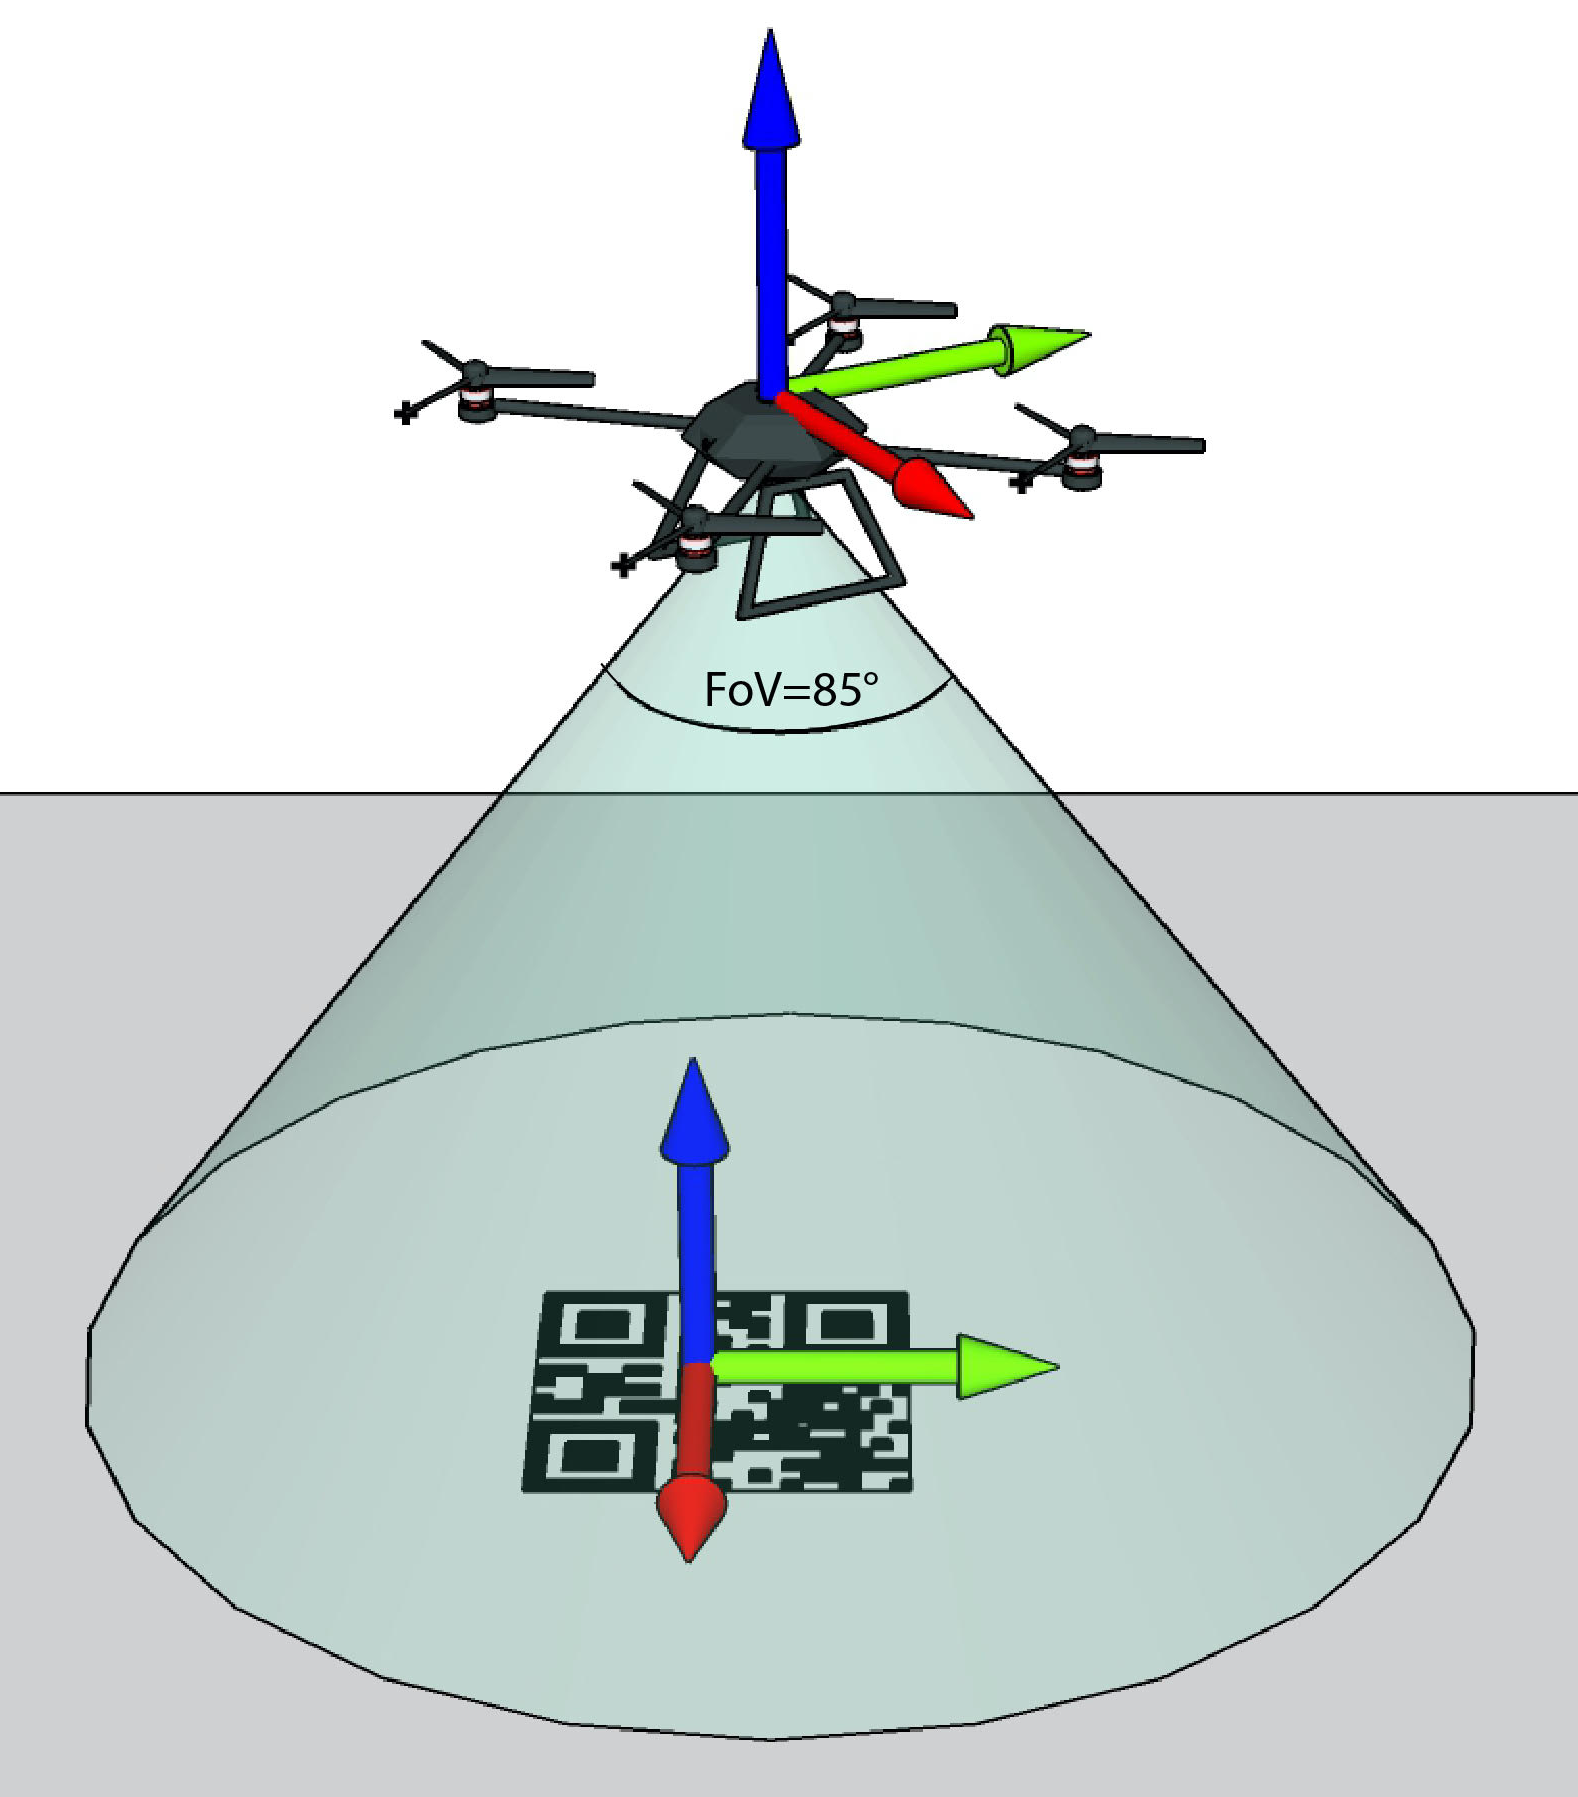
\includegraphics[width=0.5\linewidth]{Images/fig29-marker-observation.png}
    \end{frame}

    \begin{frame}[nonumber]{What about adding new markers?}
        \begin{itemize}
            \item{Inverse observation model should project the observation from the camera reference frame to the world reference frame}
            \item{Inverse observation model is then:
                \begin{align*}
                    h_i^{-1}(\hat\mu_t) =\begin{bmatrix}
                        m_{i, x}^w \\ m_{i, y}^w \\ m_{i, z}^w \\ m_{i, \phi}^w \\ m_{i, \theta}^w \\ m_{i, \psi}^w
                    \end{bmatrix} &= \bm{T_r} * \bm{T_c} * \bm{T_m}^c
                \end{align*}}
            \item{And extend the state vector:
                \begin{align*}
                    \mu_t = \left[\begin{array}{c|cccccc}
                        \mu_t & m_{i, x}^w & m_{i, y}^w & m_{i, z}^w & m_{i, \phi}^w & m_{i, \theta}^w & m_{i, \psi}^w
                    \end{array}
                    \right]^T
                \end{align*}
            and state covariance matrix}
        \end{itemize}
    \end{frame}

    \subsubsection{Height}
    \begin{frame}[nonumber]{Height}
       \begin{itemize}
           \item{The observations to correct the height are composed by the range sensor + Octomap measurement}
           \item{The height observation is $z = voxel_z + range_{distance}$}
           \item{Hence, the observation model is simply: \begin{align*}
                   h\left(\hat\mu_t\right) = \hat\mu_z + bias
           \end{align*}}
       \end{itemize}
    \end{frame}

%    \subsection{System Architecture}
%    \begin{frame}
%        This frame has an empty title.
%    \end{frame}

    %%%%%%%%%%%%%%%%%%%%
    % EXPERIMENTS
    %%%%%%%%%%%%%%%%%%%
    \section{Experiments \& Results}
    \subsection{The environment}
    \begin{frame}
        \begin{columns}[T]
            \begin{column}{.5\textwidth}
                \begin{itemize}
                    \item{Obstacles of at most 2mts height}
                    \item{6 known colored poles}
                    \item{10 unknown markers}
                    \item{10mts $\times$ 20mts}
                    \item{Delimited by net-like walls}
                \end{itemize}
            \end{column}
            \begin{column}{.5\textwidth}
                \centering
                \includegraphics[width=\linewidth,angle=90,origin=c]{Images/fig18-gazebo-environment}
            \end{column}
        \end{columns}
    \end{frame}

    \begin{frame}
        All the experiments were done in a simulated environment.\\
        The aim of the experiments were to evaluate:
        \begin{itemize}
            \item{the importance of known poles and known and unknown markers in the localization and mapping process}
            \item{the accuracy of markers' pose estimation}
            \item{the importance of the range and Octomap measurements in the height correction}
            \item{the importance of the NEES test to evaluate measurements and the filter's consistency}
        \end{itemize}
    \end{frame}
    \begin{frame}{Odometry only}
        \centering
        \includegraphics[width=0.8\linewidth]{Images/fig19-odom_only.png}
    \end{frame}

    \subsection{Experiments A}
    \begin{frame}[nonumber]{The importance of poles}
        2 experiments were carried out:
        \begin{enumerate}
            \item{using \emph{perfect observations} of poles, had the objective of showing the perfect localization compared with the MAVROS localization and the ground truth.}
            \item{using \emph{real observations} taken from the ROS bag, had the objective of understanding if the proposed implementation works as well as with the perfect observations of the previous experiment}
        \end{enumerate}
    \end{frame}

    \begin{frame}[nonumber]{Perfect observation of poles}
        \centering
        \includegraphics[width=0.7\linewidth]{Images/fig20-exp-a1.png}
    \end{frame}

    \begin{frame}[nonumber]{Real observation of poles}
        \centering
        \includegraphics[width=0.7\linewidth]{Images/fig20-exp-a2.png}
    \end{frame}

    \subsection{Experiments B}
    \begin{frame}{The importance of markers}
        3 experiments were carried out:
        \begin{enumerate}
            \item{The drone follows the path and estimates its pose based on known markers only. It had the objective of understanding the importance of markers in the localization process}
            \item{Similar to the previous one, but it uses markers and poles to localize. However, the main difference with the previous experiments lies on the absence or not of a perfect map. It had the objective of understanding the importance of both poles and markers in the SLAM situation.}
            \item{Measures the distance between the true position of markers and the one estimated by the algorithm in a context of \emph{real observations}, both for markers and poles.}
        \end{enumerate}
    \end{frame}

    \begin{frame}[nonumber]{Localization using only markers}
        \centering
        \includegraphics[width=0.7\linewidth]{Images/fig21-real-marker-wmap.png}
    \end{frame}

    \begin{frame}[nonumber]{SLAM with poles and markers}
        \centering
        \includegraphics[width=0.7\linewidth]{Images/fig22-true-poles-markers-nomap.png}
    \end{frame}
    \begin{frame}[nonumber]{Distance between real and estimated poses.}

         \centering
        \begin{tabular}{ccccc}
            \toprule
            \textsc{Marker ID} & \textsc{Euclidean distance} & \textsc{$\phi$} & \textsc{$\theta$} & \textsc{$\psi$} \\
            \midrule
            0 & 0.076 & 0.089 & 0.142 & 0.034\\
            1 & 0.186 & 0.407 & 0.145 & 0.052\\
            4 & 0.119 & 0.153 & 0.132 & 0.055\\
            5 & 0.155 & 0.024 & 0.057 & 0.013\\
            \midrule
            Max. & 0.186 & 0.407 & 0.145 & 0.055\\
            Min. & 0.076 & 0.024 & 0.057 & 0.013\\
            Avg. & 0.134 & 0.168 & 0.119 & 0.039\\
            \bottomrule
        \end{tabular}
    \end{frame}
    \subsection{Experiments C}
    \begin{frame}[nonumber]{Height estimation}
        \begin{itemize}
            \item{2 types of observations: Octomap + range sensor}
            \item{Implementation only updates height iff Octomap information is available}
            \item{1 experiment was carried out with the objective of understanding the influence of both observations in the height update.}
            \item{Real landmarks observations were used.}
        \end{itemize}
    \end{frame}
    \begin{frame}
        \centering
        \includegraphics[width=0.7\linewidth]{Images/fig23-laser-detail.png}
    \end{frame}

    \subsection{Experiments D}
    \begin{frame}{NEES test influence}
        The experiments were carried out with the objective of understanding
        \begin{enumerate}
            \item{the importance of using (or not) the NEES test}
            \item{the importance of the $\chi^2$ value}
        \end{enumerate}
    \end{frame}
    \begin{frame}{What happen when no NEES test is used?}
        \centering
        \includegraphics[width=0.65\textwidth]{Images/fig24-no-nees-test.png}
    \end{frame}

    \begin{frame}{What about the $\chi_{\alpha}^2$ threshold?}
        \begin{itemize}
            \item{So far, was used a threshold that corresponds to 95\% of valid measurements. This means that we assume that the 95\% of the observations are valid.}
            \item{This corresponds to $\alpha = 0.05$, but this value is the standard one.}
            \item{What happen with other confidence levels?}
            \item{Moreover, different thresholds can be set for different landmarks}
        \end{itemize}
    \end{frame}

    \begin{frame}{Discarded markers observations when $\alpha=0.05$}
        \centering
        \includegraphics[width=0.7\textwidth]{Images/fig24-nees-95-path-discarded-markers.png}
    \end{frame}

    \begin{frame}{Discarded markers observations when $\alpha=0.9$}
        \centering
        \includegraphics[width=0.7\textwidth]{Images/fig24-nees-10-path-discarded-markers.png}
    \end{frame}

    \begin{frame}{Height correction when $\alpha=0.9$}
        \centering
        \includegraphics[width=0.7\textwidth]{Images/fig23-laser-chi2-detail.png}
    \end{frame}


    %%%%%%%%%%%%%%%%%%%%
    % CONCLUSIONS
    %%%%%%%%%%%%%%%%%%%
    \section{Conclusions \& Future work}

    \begin{frame}[nonumber]{Conclusions}
        \begin{itemize}
            \item{The first 2 experiments showed the importance of poles and markers in the localization process.}
            \item{The markers' pose estimation in an SLAM situation is good enough for the competition context.}
            \item{The height estimation can be corrected using a combination of Octomap and range sensor.}
            \item{The completeness and correctness of the Octomap is fundamental for good results.}
            \item{NEES is fundamental for the consistency of the filter.}
            \item{Lower confidence of valid measurements implies discarding truly bad measurements, but on the other hand it can discard measurements that can be useful to correct the drone's pose.}
            \item{The value of $\alpha$ becomes a parameter of the system.}
        \end{itemize}
    \end{frame}

    \begin{frame}[nonumber]{Future work}
        \begin{itemize}
            \item{Deploy and test the proposed implementation in the real drone.}
            \item{Fine-tune the noise covariance matrices.}
            \item{Extensive experimentation with Octomap and range sensor for height update.}
            \item{Camera self calibration procedure to improve the Z position estimation using poles and markers}
            \item{Compare the current algorithm with other algorithms like Error-State EKF-SLAM, or UKF-SLAM, and evaluate their performance with the current implementation as baseline}
        \end{itemize}
    \end{frame}

    %%%%%%%%%%%%%%%%%%%%
    % QUESTIONS & THANKS
    %%%%%%%%%%%%%%%%%%%
    \section*{Questions?}
    \begin{frame}[plain]{}
        \Huge{Thank you!}
        \sectionpage
    \end{frame}



\end{document}